\documentclass[../main.tex]{subfiles}

\begin{document}
\pagebreak
\section{Description}
In this section, we will give a description of our overall system as well as a justification for our system and diagrams to support the description of the overall system.

	\subsection{Focus on properties}\label{sec: properties}
	Our system contains a lot of properties, to make all of these properties clear we use an enumeration.
	\begin{enumerate}
		\item The user can see the connection status to the server on the top right of the home screen. The user can also create a party from here and go to the settings and join a party screen.
		\item If the user's phone is disconnected to the server, then the player cannot use the create and join party buttons.
		\item Our application has a few settings: the user can change and save their name. This name will be shown in the lobby. The user can toggle btween offline/online mode using a button and the user can tobble between muted and unmuted music (heard in-game) using a button.
		\item The user can join a party by filling in the game pin of that party and clicking on enter.
		\item The user can select abilities in the lobby. The user can select three abilities which will be displayed in the game in the order they are chosen. The user can also see the master of the party, all the other party members, the ready status of the other party members and the party's game pin.
		\item If the user is the master of their party, they can start the game by pressing the button, provided all other players are ready. If the user is not the master of their party they can get (un)ready by pressing the button.
		\item The user can see the health of their character in the top right corner when in-game. This value changes in real-time when the character takes damage or is healed.
		\item When playing with multiple players, every player has a differently colored character.		
		\item While in-game, the user can walk around using the joystick and activate abilities, when they are not on a cooldown (they will appear opaque when on cooldown), using the corresponding buttons on the bottom right. 
		\item The abilities have various effects, but in our current implementation the user can teleport 4 tiles in the direction the character is facing, the user can damage other entities using arrows and a melee attack and the user can heal itself with ten health.
		\item When a player's health is displayed in the upper right corner when in-game. When it drops to zero, the player respawns at the level's spawnpoint.		
		\item The enemies fight back using their well developed A.I.
		\item When the boss is defeated, the player(s) return(s) to the lobby.
		
		\begin{figure}[H]
			\centering
					\begin{minipage}{0.45\textwidth}
						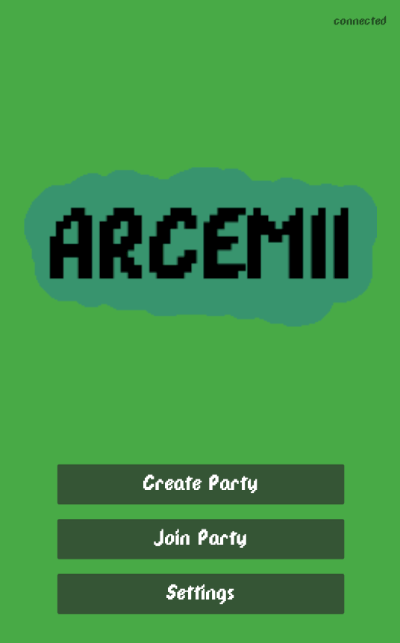
\includegraphics[height=.8\textwidth]{screenshots/main.png}
						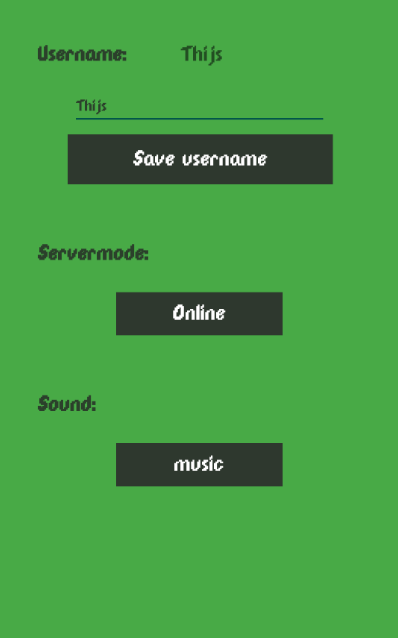
\includegraphics[height=.8\textwidth]{screenshots/settings.png}
					\end{minipage}
					\end{figure}
		\begin{figure}[H]
    	\centering
    	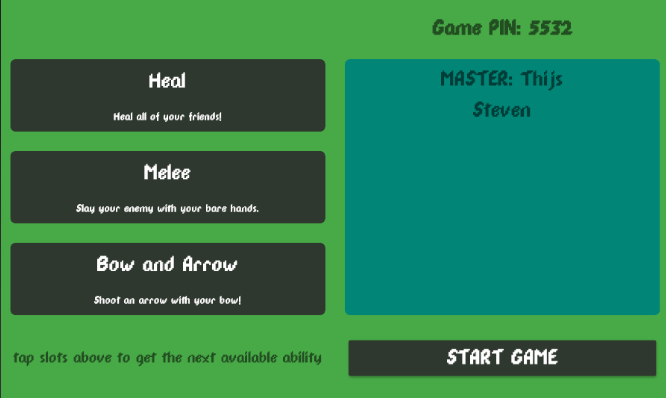
\includegraphics[height=.8\textwidth]{screenshots/party.png}
  	\end{figure}
		\begin{figure}[H]
    	\centering
    	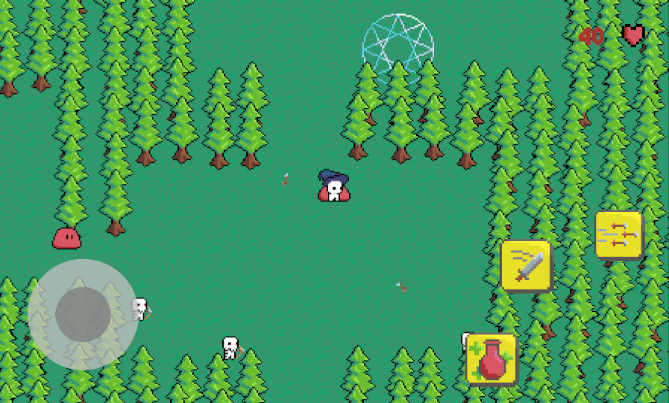
\includegraphics[height=.8\textwidth]{screenshots/game.png}
  	\end{figure}

    \end{enumerate}

	\subsection{Product justification}

	\subsection{Specifications}
	In section \ref{sec: properties}, we presented a list of properties of our application. As we'll go pretty in-depth in the next section, we decided not do that too here, as we'd only be explaining ourselves twice. 
	
	We do want to discuss some of the structures used in our code. For Reference, see sppendix \ref{fig: uml}. We decided not to expand every square present there, showing their methods and such, because the figure would become much too large and not easily readable that way.

\end{document}
